\chapter{Digital Filter Design}
	In general \de{filters} for digital signal processing are implemented in discrete-time system because, in opposition to the continuous-time one, they are easier to implement (they are in fact \textit{simple} algorithms).
	
	Given a causal discrete-time LTI system characterized by a impulse response $h(t)$, it's output to a sinusoidal input in the complex form $x(n) = A e^{j(\omega_0n+\phi_0)}$ is determined by the convolution
	\begin{equation} \label{eq:filt:shift}
	\begin{aligned} 
		y(n) & = x(n) * h(n) = \sum_{k=0}^\infty A e^{j(\omega_0(n-k)+\phi_0)}h(k) = Ae^{j\phi_0} e^{j\omega_0n} \sum_{k=0}^\infty h(k) e^{j\omega_0k} \\
		& = A e^{j(\omega_0n + \phi_0)}H\big(e^{j\omega_0}\big)
	\end{aligned}
	\end{equation}
	From this equation we can indeed see that the output of such system is still a sinusoidal function with unchanged pulsation $\omega_0$ but with a phase shift and magnitude \textit{rescalation} due to the transfer function $H$ of the system evaluated at the point $e^{j\omega_0}$ in the frequency domain. Considering the real part of the function we determine the \textit{true} output of the system as
	\[ y(n) = A \left| H\big(e^{j\omega_0}\big) \right| \cos\Big( \omega_0n + \phi_0 + \angle H\big(e^{j\omega_0}\big) \Big) \]
	where $|H(e^{j\omega})|$ is the \textbf{gain} of the system and $\angle H(e^{j\omega})$ it's \textbf{phase shift}; both parameters are evaluated for the sinusoidal pulsation $\omega_0$.	
	
	\begin{SCfigure}[2][bt]
		\centering 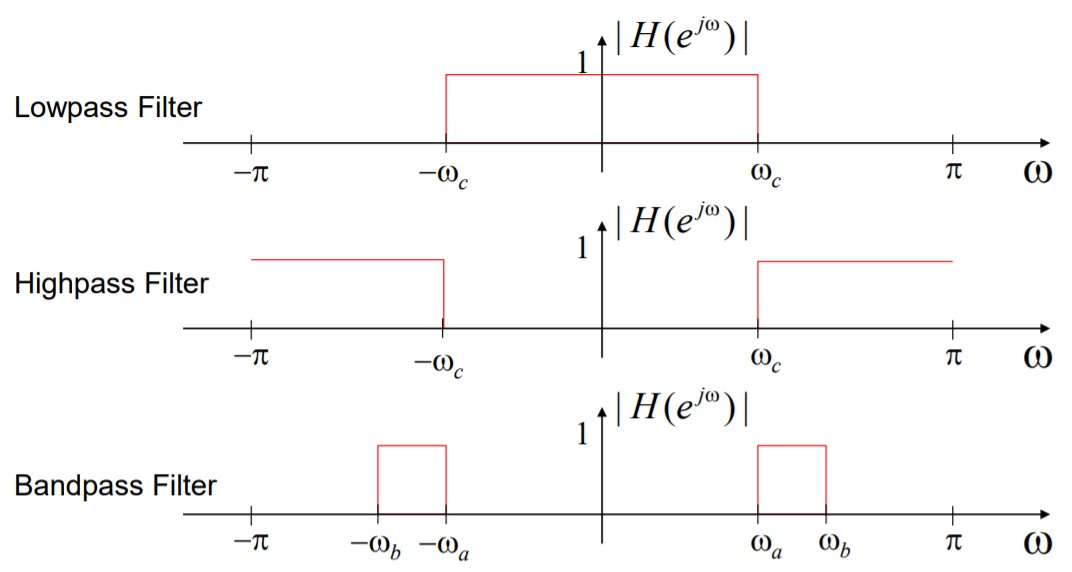
\includegraphics[width=8cm]{ideal-filters}
		\caption{examples of ideal filters in the frequency domain.}
		\label{fig:filt:idealfilter}
	\end{SCfigure}

	\paragraph{Ideal filters} Figure \ref{fig:filt:idealfilter} presents a list of the main \de{ideal filters} for discrete-time system; in particular are presented the low-pass, high-pass and band-pass filters analogous to the continuous-time ideal filters shown in section \ref{sec:conv:filters} (page \pageref{sec:conv:filters}). In practise filter with such frequency response cannot be implemented due to their \textbf{non-causality}: this kind of filters implies in fact a impulse response
	\[ h(n) \neq 0 \qquad \textrm{for } n < 0 \]
	meaning that the output should be affected by inputs that still hasn't committed.
	
	\paragraph{Low-pass filter} A low-pass filter (or any filter in general) can be practically implemented by constructing a proper window function $w(n)$ whose goal is to \textit{simulate} the spectral behaviour of the ideal counter-part. Due to the fact that they are computed on a finite number of samples $M$, the originate a distorted frequency response (respect to the ideal case) involving ripples and not-infinite slope at the cut-off frequency (as shown in figure \ref{fig:filt:windowfilter}). This ripples affect both the pass and the stop-band response due to oscillations: the pass-band gain isn't constant and the stop-band isn't univocally null.	
	
	\begin{SCfigure}[2][bht]
		\centering 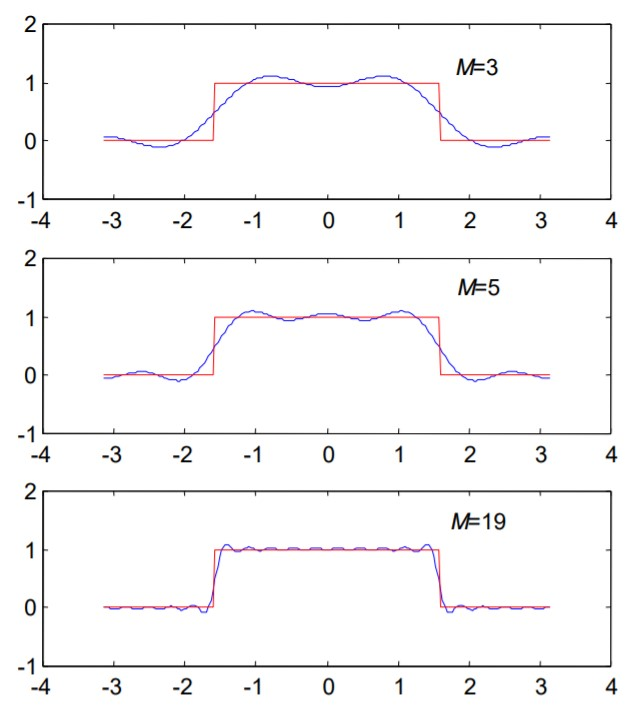
\includegraphics[width=5.5cm]{lpf-wind}
		\caption{spectral behaviour of low pass filter realised by appropriate windows of length $M$.}
		\label{fig:filt:windowfilter}
	\end{SCfigure}

\section{Filter specifications}
	In general the \textbf{design} of every \textbf{digital filter} derives by the design of a continuous-time low-pass filter. Acknowledged that an ideal implementation isn't feasible in real world application it's mandatory to define the following \de{design parameters} made on the assumption that the pass band gain is unitary:
	\begin{enumerate}[a)]
		\item the maximum deviation $\delta_1$ from the pass-band gain meaning that the real filter gain in the pass-band region must be bounded in the domain $[1-\delta_1,1]$;
		\item the maximum deviation $\delta_2$ from the 0 in the stop-band,  so ensuring that in the stop-band the gain is bounded in the set $[0,\delta_2]$;
		\item the transition bandwidth $\delta \omega$ defined as the difference of the minimum stop-band frequency $\omega_s$ and the maximum pass-band frequency $\omega_p$.
	\end{enumerate}
	
	The complete set of \textbf{specification parameters} $(\delta_1,\delta_2,\omega_p,\omega_s)$ can be synthesized in the concept of the \de{mask zone} (as shown in figure \ref{fig:filt:mask}), a graphical representation in the frequency domain of the zone that the frequency response must be stay out of (and complementary the region on which the transfer function can withstand).z
	
	\begin{SCfigure}[2][bht]
		\centering 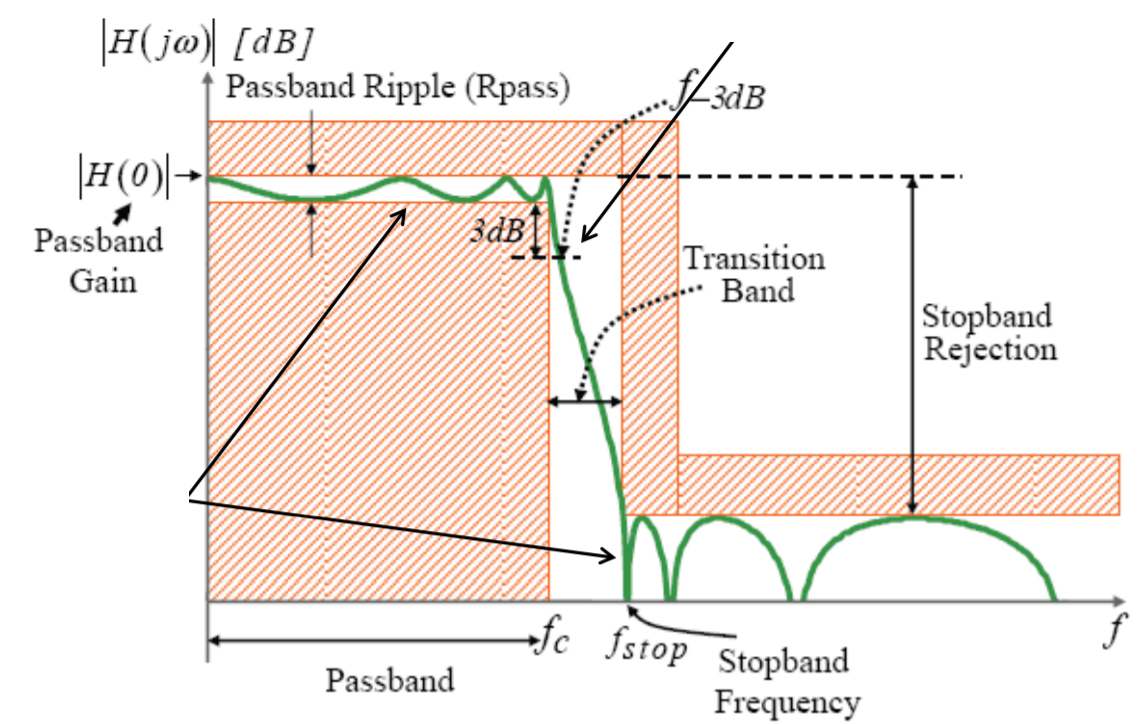
\includegraphics[width=7cm]{mask-zone}
		\caption{mask created to design a low pass filter.}
		\label{fig:filt:mask}
	\end{SCfigure}
	
	\paragraph{Phase distortion and group delay} Given a filter characterized by a impulse response $h(n)$ and transfer function $\four{h(n)} = H(e^{j\omega})$, the phase shift of a pure sinusoidal input function will be in general different depending on the phase of the system; using equation \ref{eq:filt:shift} we in fact have that
	\[ \angle H\big(e^{j\omega_1}\big) \neq \angle H\big(e^{j\omega_1}\big) \qquad \textrm{with } \omega_1 \neq \omega_2 \]
	For particular application phase distortion is relevant and should be minimized, and making it ideally constant through-out all the pass-band region; if this operation can't be achieved we can used the generalized concept of \de{group delay} $\tau_g$ defined as
	\begin{equation}
		\tau_g := - \frac{d\angle H \big(e^{j\omega}\big)}{d\omega}
	\end{equation}
	In the ideal case $\tau_g$ is constant with a value $\beta$ in the pass band meaning that, by integration, the \textbf{generalized group delay} is determined by an expression of the kind
	\[ \angle H\big(e^{j\omega}\big) = -\beta \omega + \alpha \hspace{2cm} \textrm{with } \alpha,\beta \in \mathds R \]
	
	\paragraph{Design techniques} Depending on the type of filter wanted, completely different approaches can be used, in particular
	\begin{itemize}
		\item to realize a IIR infinite impulse response filter the technique used is the approximation of standard analog filters; the main draw-back of this category of filters is that none of them has a linear phase response;		
		\item to realize an FIR finite impulse response filter two methods can be used: using particular window function or using algorithmic approaches based on optimization technique. This kind of filters can presents a generalized group delay.
	\end{itemize}

\section{IIR filter design}
	The design of any \de{discrete-time infinite impulse response filter} is based on the design of a well establisher \textbf{low-pass prototype} that's generated by following this steps:
	\begin{itemize}
		\item[0)] using \textit{bilinear transformations} the specification of a generic filter must be transformed in the specification of a single low-pass filter. This step is optional and has to be applied every-time we want to design a non-low-pass filter;		
		\item[1)] convert the discrete-time filter specifications $\omega_p,\omega_s$ into the dual analog $\Omega_p,\Omega_s$ for  continuous-time low-pass prototype;
		\item[2)] design the analog prototype considering some base reference; in the following pages Butterworth, Chebyshev I/II and elliptic filters are going to be presented;
		\item[3)] return to the discretized domain using the \textbf{impulse invariance} (not object of study) or the bilinear transform method;
		\item[4)] optionally if the filter object of study wasn't a low-pass filter, we have to apply the inverse transformation of step 0 in order to retrieve the desired filter.
	\end{itemize}
	
	\subsection{Finite difference method and bilinear transform}
		Observing that the variable $s$ in the Laplace domain corresponds to a differentiation in time and so for each $s$ present in the transfer function, the order of differentiation increases. This concept is valid for continuous-time systems however an analogy can be stated for discrete-time system the concept of derivation is interpreted by a numerical approximation; the simplest way to consider the derivative $y(n) = \frac{dx}{dn}$ can be obtained considering the definition
		\[ y(n) = \frac{x(n) - x(n-1)}{T} \]
		However numerically this solution is quite \textit{bad} and the \textbf{trapezoidal rule} is preferable having
		\begin{equation}
			\frac{y(n) + y(n-1)} 2 = \frac{x(n) - x(n-1)}{T}
		\end{equation}
		Applying the Z transform on such expression we have
		\[ \frac{Y(z) + z^{-1}Y(z)}{2} = \frac{X(z) - z^{-1}X(z)}{T} \]
		that determines the \textbf{Tustin}/\de{bilinear differentiation} as the transfer function
		\[\frac{Y(z)}{X(z)} = \frac 2 T \frac{1-z^{-1}}{1+z^{-1}} = s\]
		relating this numerical differentiation with the one in the Laplace domain characterized by the variable $s$; considering so the relations between the Z domain and the Laplace one determine by
		\begin{equation}
			s =  \frac 2 T \frac{1-z^{-1}}{1+z^{-1}} \hspace{1.2cm} \Leftrightarrow \hspace{1.2cm} z = \frac{1 + \frac T2s}{1-\frac T2s}
		\end{equation}
		it's possible to express the transfer function $H(z)$ of the discrete-time filter by knowing the continuous-time one $H_c(s)$ as
		\begin{equation} \label{eq:filt:bilinear}
			H(z) = H_c(s) \Big|_{s =  \frac 2 T \frac{1-z^{-1}}{1+z^{-1}}}
		\end{equation}
		This result is so used in the 3$^{rd}$ step of the digital filter design process in order to transform the analog prototype in the final desired filter. The first step based on transforming the filter specification from the discrete-time domain to the continuous one can be obtained by the bilinear transformation considering only the imaginary part $s=j\Omega$ of the Laplace variable:
		\begin{equation} \label{eq:filt:freqchange}
		\begin{aligned}
			j\Omega & = \frac 2 T \frac{1-e^{-j\omega}}{1+e^{j\omega}} = j \frac 2 T \frac{ e^{j\frac\omega2} - e^{-j\frac\omega2} }{e^{j\frac\omega2} + e^{-j\frac\omega2}} = j \frac 2 T \tan \left( \frac \omega 2 \right) \\
			\Omega & = \frac 2 T \tan \left( \frac \omega 2 \right) \\
			\omega & = \arctan \left( \frac{\Omega T}{2} \right)
		\end{aligned}
		\end{equation}
		Such transformation implies a \textbf{frequency warping}: the relation between the frequencies analog and discrete filters isn't linear but affected by a (arc)tangent function that preserves the integrity of the spectrum (no aliasing occurs because for $\Omega \rightarrow \pm\infty$ we obtain $\omega= \pm \pi$).
		
		
		
		
		
		
		
		
		
		
		
		
	\subsection{Butterworth filter}
		The \de{Butterworth filter} is one of the simplest system that can be design and is referred also as \textbf{\textit{maximally flat filter}}; the idea behind such filter is to have derivative up to $N$-th order (the \textbf{order} of the filter) that are nulls. The magnitude of such filter is in fact described by the equation
		\begin{equation} \label{eq:filt:magbutter}
			|H_c(\Omega)|^2 = \frac{1}{1 + \left(\frac{\Omega}{\Omega_c}\right)^{2N}}
		\end{equation} 
		where $\Omega_c$ is the \textbf{cut-off frequency} of the analog prototype. As shown in figure \ref{fig:filt:buttanalog}, the magnitude response is strictly monotonically decreasing and the \textbf{selectivity} (\textit{length} of the transition bandwidth) increases as the order $N$ grows.
		
		\begin{SCfigure}[2][bht]
			\centering 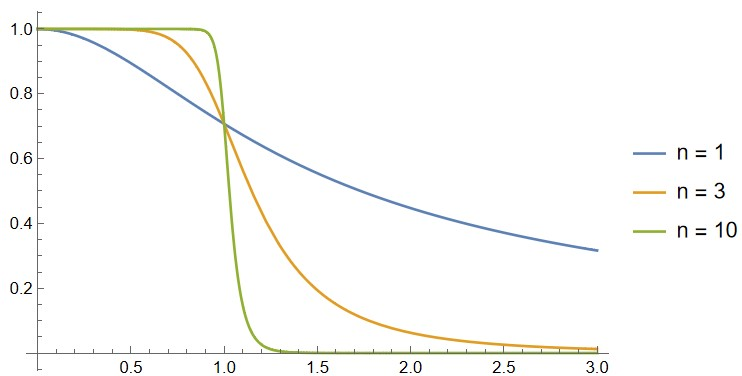
\includegraphics[width=8cm]{butter-time}
			\caption{frequency response of the Butterworth filter with cut-off frequency $\Omega_c=1$ for various order $N$.} \label{fig:filt:buttanalog}
		\end{SCfigure}
	
		The main drawback of the Butterworth filter is that it's phase distortion is strictly non-linear in the neighbourhood of the cut-off frequency (however such effect can be neglected if we are \textit{far} from such point), as shown in the Bode plots in figure \ref{fig:filt:buttbode}.	
	
		\begin{SCfigure}[2][bht]
			\centering 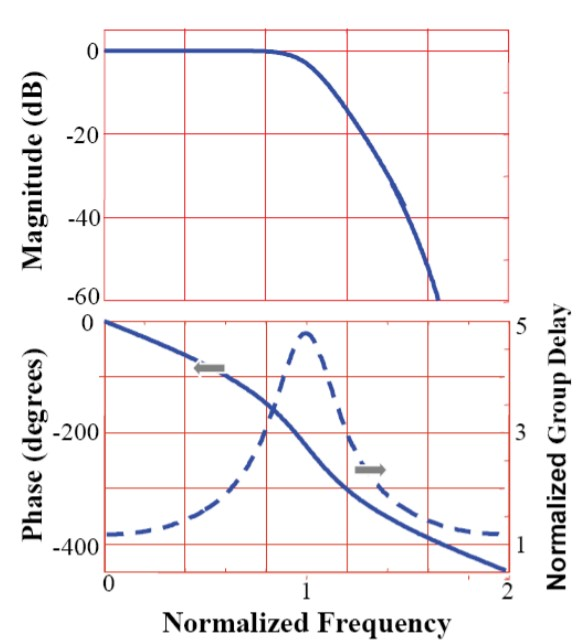
\includegraphics[width=5cm]{butter-bode}
			\caption{Bode plots of the response of the Butterworth filter.} \label{fig:filt:buttbode}
		\end{SCfigure}
		
		The \textit{complete} expression of the Butterworth frequency response can be obtained by expanding the full complex notation on equation \ref{eq:filt:magbutter}, obtaining
		\begin{equation}
			|H_c(\Omega)|^2 = H_c(s)\Big|_{s=j\Omega} H_c(-s)\Big|_{s=j\Omega} = \frac{1}{j\Omega + \left( -\frac{s}{\Omega_c} \right)^{2N}}
		\end{equation}
		This transfer function has no zeros (the numerator is just constant) and $2N$ poles lying on the unit circle on the complex plane of the variable $s$; discarding the \textit{unstable points} (the one having positive real parts) then the final poles for the Butterworth filter are described as:
		\begin{equation} \label{eq:filt:buttphase}
			\text{root's phases:} \hspace{2cm} \phi_k = \frac \pi 2 + \big(2k+1\big) \frac{\pi}{2N} \qquad \textrm{with } k=0,\dots, N-1
		\end{equation} 
	
		\subsubsection{Prototype design}
		When designing a Butterworth low-pass prototype no information are known a-priori regarding both the cut-off frequency $\Omega_c$ of the filter and it's order $N$; the only information known are the maximum/minimum deviation $\delta_1,\delta_2$  from the pass/stop-band gains and the related analog  frequencies $\Omega_p,\Omega_s$.\\
		In order to determine the parameters of the Butterworth filter we can impose that at the maximum pass-band frequency $\Omega_p$ the gain is at it's minimum value $1-\delta_1$, giving the expression
		\[ \frac 1 {1 + \left( \frac{\Omega_p}{\Omega_c} \right)^{2N}} = \big(1-\delta_1\big)^2 \]
		while at the minimum stop-band frequency $\Omega_s$ the allowed gain is $\delta_2$, hence
		\[ \frac 1 {1 + \left( \frac{\Omega_s}{\Omega_c} \right)^{2N}} = \delta_2^2 \]
	
		Solving the non-linear system determined by this two equations determines both the minimum order $N$ of the filter and the cut-off frequency $\Omega_c$ of the filter as
		\begin{equation} \label{eq:filt:butter}
			N = \left\lceil \frac{\ln \left( \dfrac{ \frac 1 {\delta_2^2} -1 }{\frac{1}{(1-\delta_1)^2}-1} \right)}{2 \ln \left(\dfrac{\Omega_s}{\Omega_p}\right)} \right\rceil \hspace{2cm} \Omega_c = \frac{\Omega_s}{\sqrt[2N]{\frac{1}{\delta_2^2}-1}}
		\end{equation}
		
		\begin{example}{: Butterworth low-pass filter design}
			Given the low-pass filter specification
			\[ \omega_p = 0.2\pi \qquad \omega_s = 0.3\pi \qquad \delta_1 = 0.10875 \qquad \delta_2 = 0.1778  \]
			the filter is designed considering the 3 main steps previously described, and in particular:
			\begin{enumerate}
				\item the first thing is to convert the digital filter specification into analog ones in order to build the matching prototype; in order to do so we have to consider the bilinear transform as in equation \ref{eq:filt:freqchange} where the sampling time $T$ is arbitrarily chosen to be 1, and so
				\[ \Omega_p = 2\tan\left( \frac{\omega_p}{2} \right) =0.6498 rad/s \qquad \Omega_s = 2\tan \left( \frac{\omega_s}{2} \right) = 1.019 rad/s \]
				
				\item with the specification of the low-pass prototype stated it's possible to use equation \ref{eq:filt:butter} to determine the minimum order $N$ of the filter as
				\[ N = \left\lceil \frac{\ln \left( \dfrac{\frac{1}{0.1778^2}-1}{\frac 1{0.89^2}-1} \right) }{2 \ln\left(\dfrac{1.019}{0.6498}\right)} \right\rceil = \big\lceil 5.3 \big\rceil = 6 \] 
				and so the cut-off frequency
				\[ \Omega_c = \frac{1.019}{\sqrt[12]{\frac{1}{0.1778^2}-1}} = 0.7662 rad/s \]
				With this parameters defined it's possible to compute the roots of the filter as $s_k = \Omega_c \big(\cos\phi_k \pm j \sin \phi_k\big)$ where $\phi_k$ was defined in equation \ref{eq:filt:buttphase} and we obtain
				\[ s_{0,5} = -0.198 \pm j 0.74 \qquad s_{1,4} = -0.54 \pm j 0.54 \qquad s_{2,3} = -0.74 \pm j 0.198 \] 
				Considering the expansion $(s-s_k)(s-s_k^*) = s^2- 2s\Re{s_k} + |s_k|^2$ and that $|s_k|= \Omega_c$ then the formulation in the Laplace domain of the low-pass prototype is
				\[ H_c(s) = \frac{H_0}{\prod_{k=0}^{N-1} (s-s_k) } = \frac{0.202}{ (s^2 + 0.397s + 0.587)(s^2+1.085s+0.587)(s^2+1.185s + 0.587) } \]
				where $\Omega_0$ was determined as $\prod_{k=0}^{5} s_k = \Omega_c^2 = 0.202$.
				
				\item using now the bilinear transform (equation \ref{eq:filt:bilinear}) it's possible to re-convert the analog prototype  (in the Laplace domain) onto the corresponding discrete-time low-pass filter; considering that each complex root is transformed as
				\[ s^2 + \alpha_k s + \beta_k\Big|_{s =  \frac 2 T \frac{1-z^{-1}}{1+z^{-1}}} = \frac{1- A_k z^{-1} + B_kz^{-2}}{C_k \big(1+z^{-1}\big)^2} \]
				where
				\[ A_k = \frac{8-2\beta_k}{4+2\alpha_k + \beta_k} \qquad B_k = \frac{4-2\alpha_k + \beta_k}{4 + 2\alpha_k +\beta_k} \qquad C_k = \frac 1 {4+2\alpha_k + \beta_k} \]
				With that said the transfer function so becomes
				\begin{align*}
					H(z) & = \frac{\big(1+z^{-1}\big)^6 C_0C_1C_2 H_0}{ \big(1 - A_0 z^{-1} + B_0z^{-2}\big) \big(1 - A_1 z^{-1} + B_1z^{-2}\big) \big(1 - A_2 z^{-1} + B_2z^{-2}\big) } \\
					& = \frac{\big(1+z^{-1}\big)^6 0.186\cdot 0.148\cdot 0.144 \cdot 0.2022}{ \big(1 - 1.268 z^{-1} + 0.705z^{-2}\big) \big(1 - 1.012 z^{-1} + 0.36z^{-2}\big) \big(1 - 0.981 z^{-1} + 0.319z^{-2}\big) }
				\end{align*}
				
				
				
				
			\end{enumerate}
		\end{example}
		
	\subsection{Chebyshev type I}
		The \de{Chebyshev} of filter of the \de{first type} presents one more additional parameter: the \textbf{maximum ripple amplitude} $\varepsilon$ that determines the magnitude response of the form
		\begin{equation} \label{eq:filt:cheby1}
			\big|H_c(\Omega)\big|^2 = \frac{1}{1 + \varepsilon^2 P_N^2 \big(\Omega/\Omega_c\big)}
		\end{equation}
		where $P_N(x)$ is the \textbf{Chebyshev polynomial} of order $N$ formally defined as $P_N(x) = \cos\big(N\arccos x\big)$; expanding it's definition and making some analytical simplification we have
		\[ P_0(x) = 1 \qquad P_1(x) = x \qquad P_2(x) = 2x^2-1 \qquad P_3(x) = 4x^3-3x \]
		We can see so that, starting from the first 2 polynomials, the other can be computed considering the recursive definition $P_N(x) = 2x P_{N-1}(x) - P_{N-2}(x)$.
		
		\begin{SCfigure}[2][bt]
			\centering 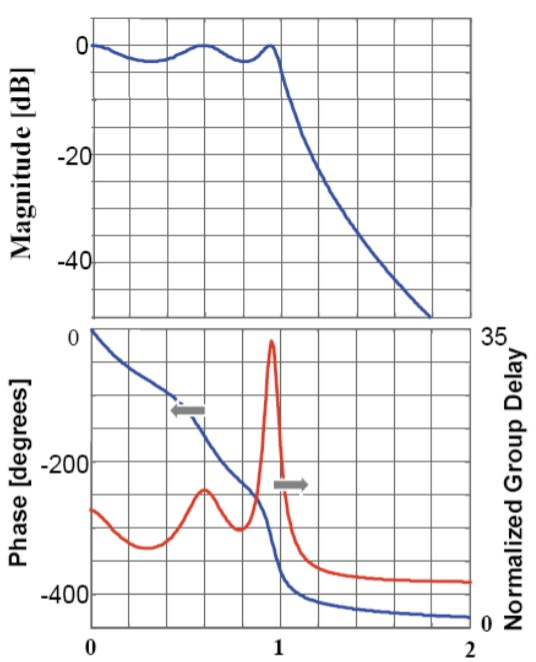
\includegraphics[width=5cm]{cheby-1}
			\caption{Bode plots of the response of the Chebyshev type I filter.} \label{fig:filt:cheby-1bode}
		\end{SCfigure}
		
		As shown in figure \ref{fig:filt:cheby-1bode} this kind of filter is characterized by an \textbf{equi-ripple} behaviour (the ripples have the same \textit{amplitude}) in the pass-band with a ripple amplitude equal to $\varepsilon$ while no ripples are present in the stop-band; this phenomena leads to a severe phase distortion in the same region but this kind of filter, for the same order $N$, has a \textit{sharper} transition bandwidth meaning that's more selective.
		
		By doing a full analysis of equation \ref{eq:filt:cheby1} it can be observed that the function still has no zeros but have $2N$ poles lying on an ellipse in the complex plane with a major diameter belonging to the imaginary axis ranging from $-j$ to $j$. To position of the poles is defined by equation
		\begin{equation}
			s_k = r_1 \cos\phi_k + j r_2 \sin\phi_k \hspace{2cm} k = 0,\dots, N-1
		\end{equation}
		where
		\[ r_1 = \frac 1 2 \left( \sqrt[N]\alpha - \sqrt[N]{\frac 1 \alpha} \right) \qquad r_2 = \frac 1 2 \left( \sqrt[N]\alpha + \sqrt[N]{\frac 1 \alpha} \right) \qquad \alpha = \frac 1 \varepsilon + \sqrt{1 + \frac{1}{\varepsilon^2}} \qquad \phi_k = \frac \pi 2 + (2k+1) \frac \pi {2N} \]
	
		\subsubsection{Prototype design}
		In the design of the prototype the first step is to relate the maximum deviation $\delta_1$ in the pass-band region with the maximum ripple amplitude parameter $\varepsilon$ that's so determined by the expression
		\begin{equation}
			1 - \delta_1 = \frac{1}{\sqrt{1+\varepsilon^2}} \hspace{1.2cm} \Rightarrow \hspace{1.2cm} \varepsilon = \sqrt{\frac 1 {\big(1-\delta_1\big)^2} - 1}
		\end{equation}
		By applying similar boundary conditions stated on the prototype design of the Butterworth filter we can obtain the minimum order $N$ of the filter as
		\begin{equation}
			N = \left\lceil \frac{\ln\left( \dfrac{\sqrt{1-\delta_2^2} + \sqrt{1-\delta_2^2(1+\varepsilon^2)}}{\varepsilon\delta_2} \right)}{\ln\left( \dfrac{\Omega_s}{\Omega_p} + \sqrt{\left( \dfrac{\Omega_s}{\Omega_p} \right)^2 - 1} \right)} \right\rceil
		\end{equation}
		In this case the cut-off frequency of the filter coincides with the maximum pass-band frequency, so $\Omega_c=  \Omega_p$.
	
	\subsection{Examples}
		\begin{example}{: IIR filter design}
			The goal is to design a Butterworth discrete-time low pass filter with specifications:
			\begin{itemize}
				\item magnitude ripple of no more than $0.2dB$ for $|\omega|\leq \frac \pi 6$;
				\item stop-band attenuation of at least $25dB$ for $|\omega| \geq 0.45\pi$.
			\end{itemize}
			To solve this problem:
			\begin{enumerate}
				\item firstly we have to determine the specification of the filter in the linear domain; considering the magnitude ripple we obtain the maximum deviation $\delta_1$ as
				\begin{align*}
					20 \log_{10}(1-\delta_1) = -0.2 \qquad \Rightarrow \qquad \delta_1 & = 1 - 10^{-\frac{0.2}{20}} = 0.0227 \\
					1-\delta_1 &= 0.977
				\end{align*}
				while for the minimum deviation
				\[ 20\log_{10}\delta_2 = - 25 \qquad \Rightarrow \qquad \delta_2 = 10^{-\frac{25}{20}} = 0.056 \]
				Assuming a sampling period $T=1$, the warped frequency for the continuous-time prototype obtained by equation \ref{eq:filt:freqchange} are
				\[ \Omega_p = 2 \tan\left( \frac{\pi/6}2 \right) = 0.536 rad/s \qquad \Omega_s = 2 \tan\left( \frac{0.45\pi}{2} \right) = 1.708 rad/s  \]
				
				\item with the specification converted for the low-pass prototype, using equation \ref{eq:filt:butter} it's possible to compute the minimum order $N$ of the system 
				\[ N = \left\lceil \frac{\ln \left( \dfrac{ \frac 1 {0.056^2} -1 }{\frac{1}{0.977^2}-1} \right)}{2 \ln \left(\dfrac{1.708}{0.536}\right)} \right\rceil = \big\lceil   3.8 \big\rceil = 4\]
				and so the cut-off frequency
				\[ \Omega_c = \frac{1.708}{\sqrt[8]{\frac{1}{0.056^2}-1}} = 0.831 rad/s \]
				The poles of the transfer function are so characterized by the formulation $s_k = \Omega_c\big(\cos\phi_k \pm k \sin\phi_k\big)$ where $\phi_k = \frac \pi 2 + (2k+1)\frac{\pi}{2N}$ and so the poles are
				\[ s_{0,3} = -0.318 \pm j0.768 \hspace{1.5cm} s_{1,2} = -0.768 \pm j 0.318 \]
				Knowing that $(s-s_k)(s-s_k^*) = s^2 -2s\Re{s_k} + |s_k|^2$ and that $H_0 = \Omega_c^4 = 0.831^4 = 0.477$ we have the following transfer function:
				\[ H_c(s) = \frac{0.477}{(s^2 + 0.636s +0.69)(s^2 + 1.536s + 0.69)} \]
				
				\item for transform the continuous-time prototype in the discrete-time filter we have to apply the bilinear transform (equation \ref{eq:filt:bilinear}); knowing that
				\[ s^2 + \alpha_k s_k +\beta_k\Big|_{s=\frac 2 T\frac{1-z^{-1}}{1+z^{-1}}} = \frac{1 + A_kz^{-1} + B_k z^{-2}}{C_k(1-z^{-1})^2} \]
				where
				\[ A_k = \frac{2\beta_kT  - 8}{4+2\alpha_kT + \beta_kT} \qquad  B_k = \frac{4 - 2\alpha_k T + \beta_k T}{4+2\alpha_kT + \beta_kT} \qquad C_k = \frac{T^2}{4+2\alpha_kT + \beta_kT} \]
				then the discrete-time filter's transfer function is
				\begin{align*}
					H(z) & = \frac{H_0(1-z^{-1})^4 C_0C_1}{\big(1 + A_0z^{-1} + B_0z^{-2}\big) \big(1 + A_1z^{-1} + B_1z^{-2}\big) } \\
					& = \frac{0.477 \cdot 0.168 \cdot 0.129 (1-z^{-1})^4}{\big(1 - 1.11z^{-1} + 0.573z^{-2}\big) \big(1 - 0.853z^{-1} + 0.208z^{-2}\big) }\\
					& = \frac{ 0.0103 (1-z^{-1})^4 }{ 1 - 1.963z^{-1} - 1.727 z^{-2} - 0.719 z^{-3} +0.119 z^{-4}  }
				\end{align*}
			\end{enumerate}
			If instead we would have considered a Chebyshev filter of the first type the minimum order required for the filter is lower than the Butterworth filter due to it's higher selectivity; determined the maximum amplitude ripple
			\[ \varepsilon = \sqrt{\frac{1}{0.977^2}-1} = 0.218 \]
			the minimum order of the filter is computed as
			\[ N = \left\lceil \frac{ \ln\left( \dfrac{\sqrt{1-0.056^2} + \sqrt{1-0.056^2(1+0.218^2)} }{0.281\cdot 0.056} \right) }{\ln \left( \dfrac{1.708}{0.536} + \sqrt{\left( \dfrac{1.708}{0.536} \right)^2-1} \right)} \right\rceil = \big\lceil 2.79 \big\rceil = 3 \]
			
		\end{example}
	
	
	